\documentclass[]{article}

%%%%%%%%%%%%%%%%%%%
% Packages/Macros %
%%%%%%%%%%%%%%%%%%%
\usepackage{amssymb,latexsym,amsmath}     % Standard packages
\usepackage{graphicx}

%%%%%%%%%%%
% Margins %
%%%%%%%%%%%
\addtolength{\textwidth}{1.0in}
\addtolength{\textheight}{1.00in}
\addtolength{\evensidemargin}{-0.75in}
\addtolength{\oddsidemargin}{-0.75in}
\addtolength{\topmargin}{-.50in}


%%%%%%%%%%%%%%%%%%%%%%%%%%%%%%
% Theorem/Proof Environments %
%%%%%%%%%%%%%%%%%%%%%%%%%%%%%%
\newtheorem{theorem}{Theorem}
\newenvironment{proof}{\noindent{\bf Proof:}}{$\hfill \Box$ \vspace{10pt}}  


%%%%%%%%%%%%
% Document %
%%%%%%%%%%%%
\begin{document}

\title{CS 224n Assignment 2.}
\author{Abhishek Goswami.}
\maketitle

\begin{enumerate}
	\item Written : Understanding word2vec
	
	\begin{enumerate}
		
		\item
		% (a) question on cross entropy
		\begin{equation}
		\sum_{w \in Vocab} y_w \log(\hat{y}_w) = - \log(\hat{y}_o).
		\end{equation}

		because
		
		\begin{equation}
		y_{i} = 
\begin{cases}
    1, & \text{if } i = o\\
    0, & \text{otherwise}
\end{cases}.
		\end{equation}
			
		\item
		% (b) question to compute wrt v_{c}
		\begin{equation}
		{\partial 		\boldsymbol{J}_\textsubscript{naive-softmax}(\boldsymbol{\upsilon}_c, o, \boldsymbol{U}) \over \partial \boldsymbol{\upsilon}_c} = 
		- \boldsymbol{u}_{o} + \sum_{w=1}^V \hat{y}_w \boldsymbol{u}_{w}.
		\end{equation}

		also equivalent to 
		
		\begin{equation}
		{\partial 		\boldsymbol{J}_\textsubscript{naive-softmax}(\boldsymbol{\upsilon}_c, o, \boldsymbol{U}) \over \partial \boldsymbol{\upsilon}_c} = 
		\boldsymbol{U} (\boldsymbol{\hat{y}} - \boldsymbol{y}).
		\end{equation}
		
		\item
		%  (c) question to compute wrt U
		\begin{equation}
		{\partial 		\boldsymbol{J}_\textsubscript{naive-softmax}(\boldsymbol{\upsilon}_c, o, \boldsymbol{U}) \over \partial \boldsymbol{U}} = 
		\boldsymbol{v}_{c} (\boldsymbol{\hat{y}} - \boldsymbol{y})^\top.
		\end{equation}
	
		also equivalent to 
		
		\begin{equation}
		{\partial 		\boldsymbol{J}_\textsubscript{naive-softmax}(\boldsymbol{\upsilon}_c, o, \boldsymbol{U}) \over \partial \boldsymbol{U}}= 
\begin{cases}
    (\hat{y}_{w} - 1) \boldsymbol{\upsilon}_c, & \text{if } x\geq 1\\
    \hat{y}_{w} \boldsymbol{\upsilon}_c, & \text{otherwise}
\end{cases}.
		\end{equation}
		
		\item
		%  (d) derivative of sigmoid. 
		\begin{equation}
		\sigma^{\prime}(\boldsymbol{x}) = \sigma(\boldsymbol{x}) (1 - \sigma(\boldsymbol{x}))
		\end{equation}
		
		\item
		%  (e) derivative of neg sample.
		\begin{equation}
		{\partial 		\boldsymbol{J}_\textsubscript{neg-sample}(\boldsymbol{\upsilon}_c, o, \boldsymbol{U}) \over \partial \boldsymbol{\upsilon}_c} = 
		(\sigma(\boldsymbol{u}_{o}^\top \boldsymbol{v}_c) - 1) \boldsymbol{u}_{o} -
		\sum_{k=1}^{k} (\sigma(\boldsymbol{u}_{k}^\top \boldsymbol{v}_c) - 1) \boldsymbol{u}_{k}
		\end{equation}

		\begin{equation}
		{\partial 		\boldsymbol{J}_\textsubscript{neg-sample}(\boldsymbol{\upsilon}_c, o, \boldsymbol{U}) \over \partial \boldsymbol{u}_c} = 
		(\sigma(\boldsymbol{u}_{o}^\top \boldsymbol{v}_c) - 1) \boldsymbol{v}_{c}.
		\end{equation}
		
		\begin{equation}
		{\partial 		\boldsymbol{J}_\textsubscript{neg-sample}(\boldsymbol{\upsilon}_c, o, \boldsymbol{U}) \over \partial \boldsymbol{u}_k} = 
		-(\sigma(-\boldsymbol{u}_{k}^\top \boldsymbol{v}_c) - 1) \boldsymbol{v}_{c}.
		\end{equation}
		
		\item
		%  (f) skip gram.
		
		\begin{enumerate}
			\item 
			
		\begin{equation}
		{\partial 		\boldsymbol{J}_\textsubscript{skip-gram}(\boldsymbol{\upsilon}_c, w_{t-m},... w_{t+m}, \boldsymbol{U}) \over \partial \boldsymbol{U}} = 
		\sum_{-m \leq j \leq m, j \neq 0} {\partial 		\boldsymbol{J}(\boldsymbol{\upsilon}_c, w_{t+j}, \boldsymbol{U}) \over \partial \boldsymbol{U}}.
		\end{equation}
		
      \item
	
		\begin{equation}	
		{\partial 		\boldsymbol{J}_\textsubscript{skip-gram}(\boldsymbol{\upsilon}_c, w_{t-m},... w_{t+m}, \boldsymbol{U}) \over \partial \boldsymbol{\upsilon}_{c}} = 
				\sum_{-m \leq j \leq m, j \neq 0} {\partial 		\boldsymbol{J}(\boldsymbol{\upsilon}_c, w_{t+j}, \boldsymbol{U}) \over \partial \boldsymbol{v}_{c}}
		\end{equation}	
			
			\item 
		
		\begin{equation}	
		{\partial 		\boldsymbol{J}_\textsubscript{skip-gram}(\boldsymbol{\upsilon}_c, w_{t-m},... w_{t+m}, \boldsymbol{U}) \over \partial \boldsymbol{\upsilon}_{w}} = 0, 
		\text{when} w \neq c
		\end{equation}
			
    \end{enumerate}
  
	\end{enumerate}

	\item Coding
	
	\begin{figure}
    \centering
    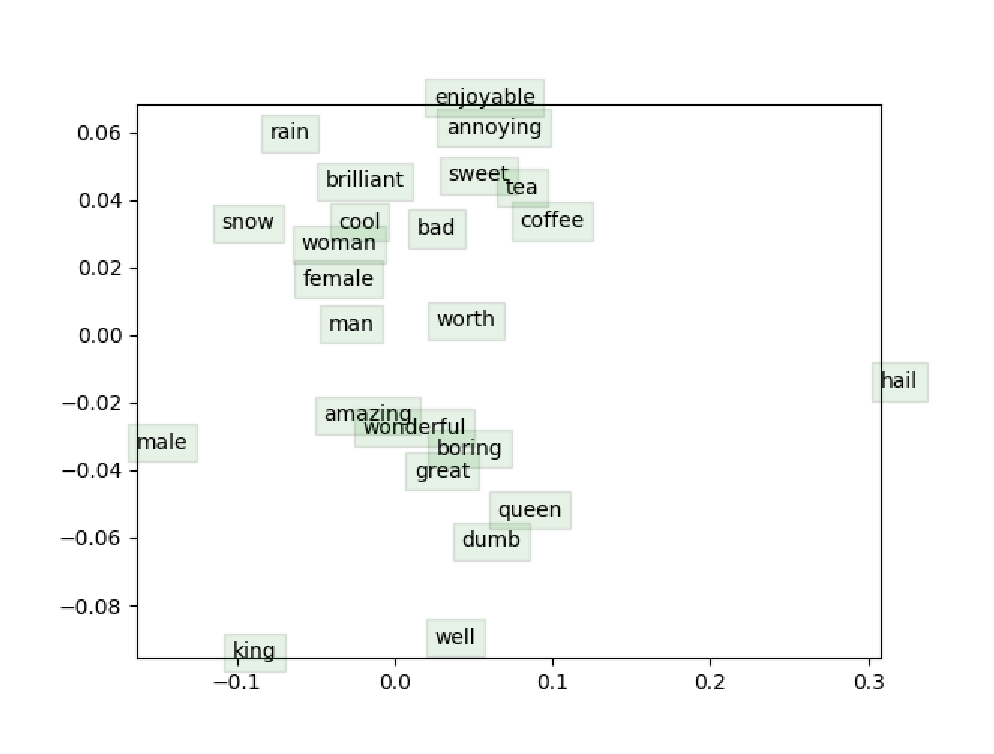
\includegraphics{word_vectors}
    \caption{Word Vectors}
    \label{word_vectors}
	\end{figure}
	
\end{enumerate}

\end{document}